\chapter{Versiju vadība}

% Ievadiņš

Šajā darba nodaļā apskatīta versiju vadības sistēmu jeb VCS\nomenclature{VCS}{versiju vadības sistēma (angl. \textit{Version control system})} vēsture un pielietojums. VCS galvenais uzdevums ir saglabāt laika gaitā veiktās izmaiņas, kas veiktas ar datnēm. VCS ļauj arī atmest laika gaitā veiktās izmaiņas, atgriezties iepriekšējā stāvoklī, salīdzināt izmaiņas, redzēt kurš un kad ir veicis izmaiņas, kas atvieglo kļūdu atrašanu un to izlabošanu. Izmantojot VCS ir daudz grūtāk veikt neatgriezeniskas izmaiņas, piemēram, kļūdas pēc izdzēstu datni ir iespējams viegli atgūt.

\section{Versiju vadības sistēmu vēsture}
VCS iedalās trīs paudzēs. Pirmās paudzes VCS bija datņu orientētas un lokālas. Lielākā daļa no tām strādāja sprostojot (angl. \textit{locking}) datnes, tā liedzot laiksakritīgu (angl. \textit{concurrent}) darbu.
Otrās paudzes VCS ir centralizētas un tās strādā uz sapludināšanas (angl. \textit{merging}) principa.
Trešās paudzes VCS ir veidotas decentralizētas, tās arī strādā pēc sapludināšanas principa.
\cite[history]{raymondVCS}
% \cite[chapter, p.~27]{chacon2014progit}
% No ProGit book
% Kad, kāpēc, kā strādā?
\subsection{Lokālas versiju vadības sistēmas}
Visvienkāršākā VCS, ko cilvēki mēdz izmantot ir vienkārša datņu pārkopēšana no vienas mapes citā, vai arī arhīvu veidošana. Šāds variants ir diezgan nedrošs, jo pieļauj cilvēcīgas kļūdas, piemēram, nepareizas datnes izmainīšanu. Tāpēc programmētāji radīja lokālu VCS, kas vienkāršā datubāzē saglabāja veiktās izmaiņas. Lokālu VCS darbības princips attēlā \ref{fig:VersionControlLocal}.
\begin{figure}[H]%!ht
	\centering
	\captionsetup{justification=centering}
	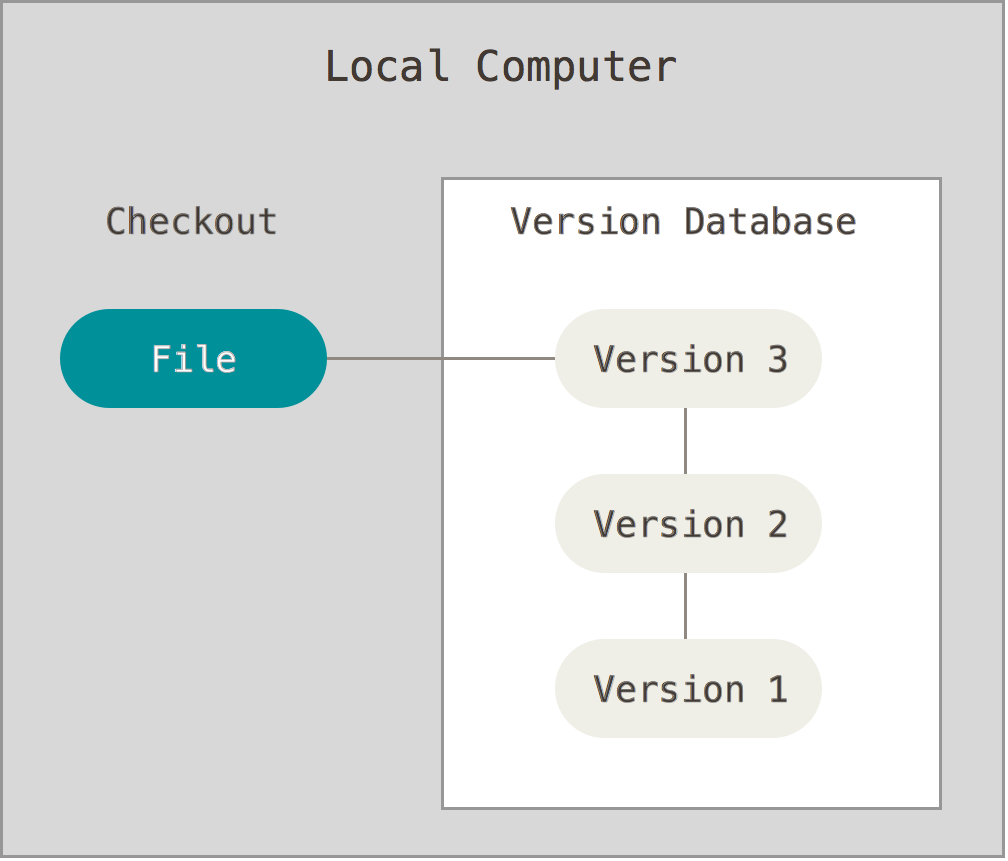
\includegraphics[width=0.5\textwidth]{VersionControlLocal.png}
	\caption{Lokālas VCS struktūras princips\ref{appfig:VersionControlLocal}}
	\label{fig:VersionControlLocal}
\end{figure}
Pirmā VCS bija \textit{Source Code Control System} (\textit{SCCS}), ko 1972. gadā uzrakstīja \textit{Marc Rochkind}, viens no Bell Labs izstrādātājiem. Tā tika radīta priekš IBM lieldatoriem (angl. \textit{mainframe}) un bija speciāli paredzēta programmatūrai un skaidri definēja versiju vēsturi. \textit{SCCS} ieviesa galvenās (angl. \textit{major} un papildversijas (angl. \textit{minor}) numurēšanu.
Otrā VCS, kas tika radīta ir \textit{GNU Revision Control System} (\textit{RCS}) un tiek vēl izmantota mūsdienās. Tā tika radīta 1980' gadu sākumā un darbojas pēc līdzīga principa kā SCCS. \texit{RCS} ir viegla un ar mazu virstēriņu (angl. \textit{low-overhead}), salīdzinot ar vēlākām un spējīgākām VCS.

\subsection{Centralizētas VCS}
Lokālas VCS ir lieliskas, lai atvieglotu viena izstrādātāja darbu, bet ar lokālām VCS ir grūti vairākiem cilvēkiem sadarboties. Lai to atrisinātu tika radītas centralizētas VCS jeb CVCS\nomenclature{CVCS}{Centralizēta versiju vadības sistēma (angl. \textit{Centralized Version Control System})}. Šādām sistēmām, piemēram CVS, Subversion un Perforce, ir viens serveris uz kura atrodas visas datnes un no kura vairāki klienti tās paņem. Salīdzinot ar lokālām VCS, šādi būtiski uzlabojas spēja sadarboties. Tomēr CVCS sistēmām ir arī būtiskas problēmas. Visas datņu versijas atrodas tikai un vienīgi uz servera, bet klientam ir tikai tā versija, kuru tas paņēmis. Tāpēc, ja centrālais serveris atsakās darboties, izstrādātāju darbs praktiski tiek paralizēts, jo nav iespējams paņemt vai iesūtīt (angl. \textit{commit}) savas izmaiņas. Ja uz centrālā servera rodas datu bojājumi, ir iespējams pazaudēt visu projekta vēsturi, ja nav veikta VCS datubāzes dublēšana.
CVCS atvieglo sadarbību, bet tās centralizētais raksturs pieļauj projekta vēstures zaudēšanu, jo klientam ir tikai tā versija, ko tas paņēmis no centrālā servera. CVCS struktūra attēlā \ref{fig:VersionControlCentralized}.
\begin{figure}[H]%!ht
	\centering
	\captionsetup{justification=centering}
	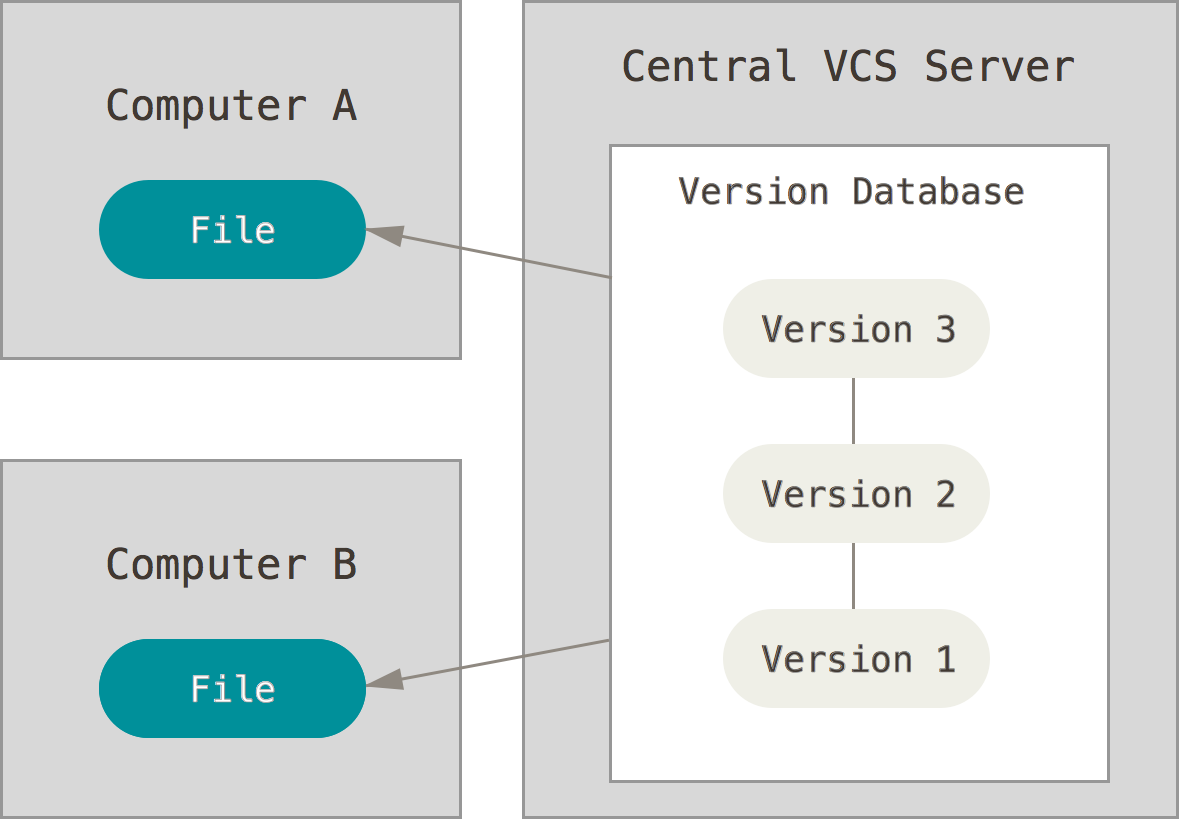
\includegraphics[width=0.5\textwidth]{VersionControlCentralized.png}
	\caption{Centralizētas VCS \ref{appfig:VersionControlCentralized}}
	\label{fig:VersionControlCentralized}
\end{figure}
Pirmais CVCS piemērs ir \textit{Concurrent Version System} (\textit{CVS}). Tā guva popularitāti ap 1990. gadu. Datu saglabāšanai tā izmanto \textit{RCS}, bet \textit{CVS} ieviesa jaunas idejas, lai izstrādātāji varētu sadarboties. Tikai ieviests sapludināšanas princips, kā arī centralizēts serveris, uz kura glabājas repozitorijs.
Populārākā un labākā CVCS ir \textit{Apache Subversion} (\textit{SVN}). Tās pirmā stabilā versija tika izdota 2004. gadā. SVN izmanto līdzīgu, tīrāku terminoloģiju nekā CVS un ir daudz stabilāka, kā arī spējīgāka par to.

\subsection{Dalītas VCS}
CVCS problēmas atrisina dalītas VCS jeb DVCS\nomenclature{DVCS}{dalīta versiju vadības sistēma (angl. \textit{Distributed Version Control System})}. DCVS sistēmās, kā Git, Mercurial, Bazaar, Darcs joprojām izmanto centralizētu serveri, uz kura klienti iesūta savas izmaiņagrāmatass, bet atšķirībā no CVCS, klienti nepaņem tikai datņu pēdējās versijas, bet pilnībā visu projekta vēsturi. Tādejādi, galvenajam serverim atsaktoties darboties, projekta vēsturi ir iespējams atjaunot no jebkura klienta. DVCS struktūra attēlā \ref{fig:VersionControlDistributed}.
\begin{figure}[H]%!ht
	\centering
	\captionsetup{justification=centering}
	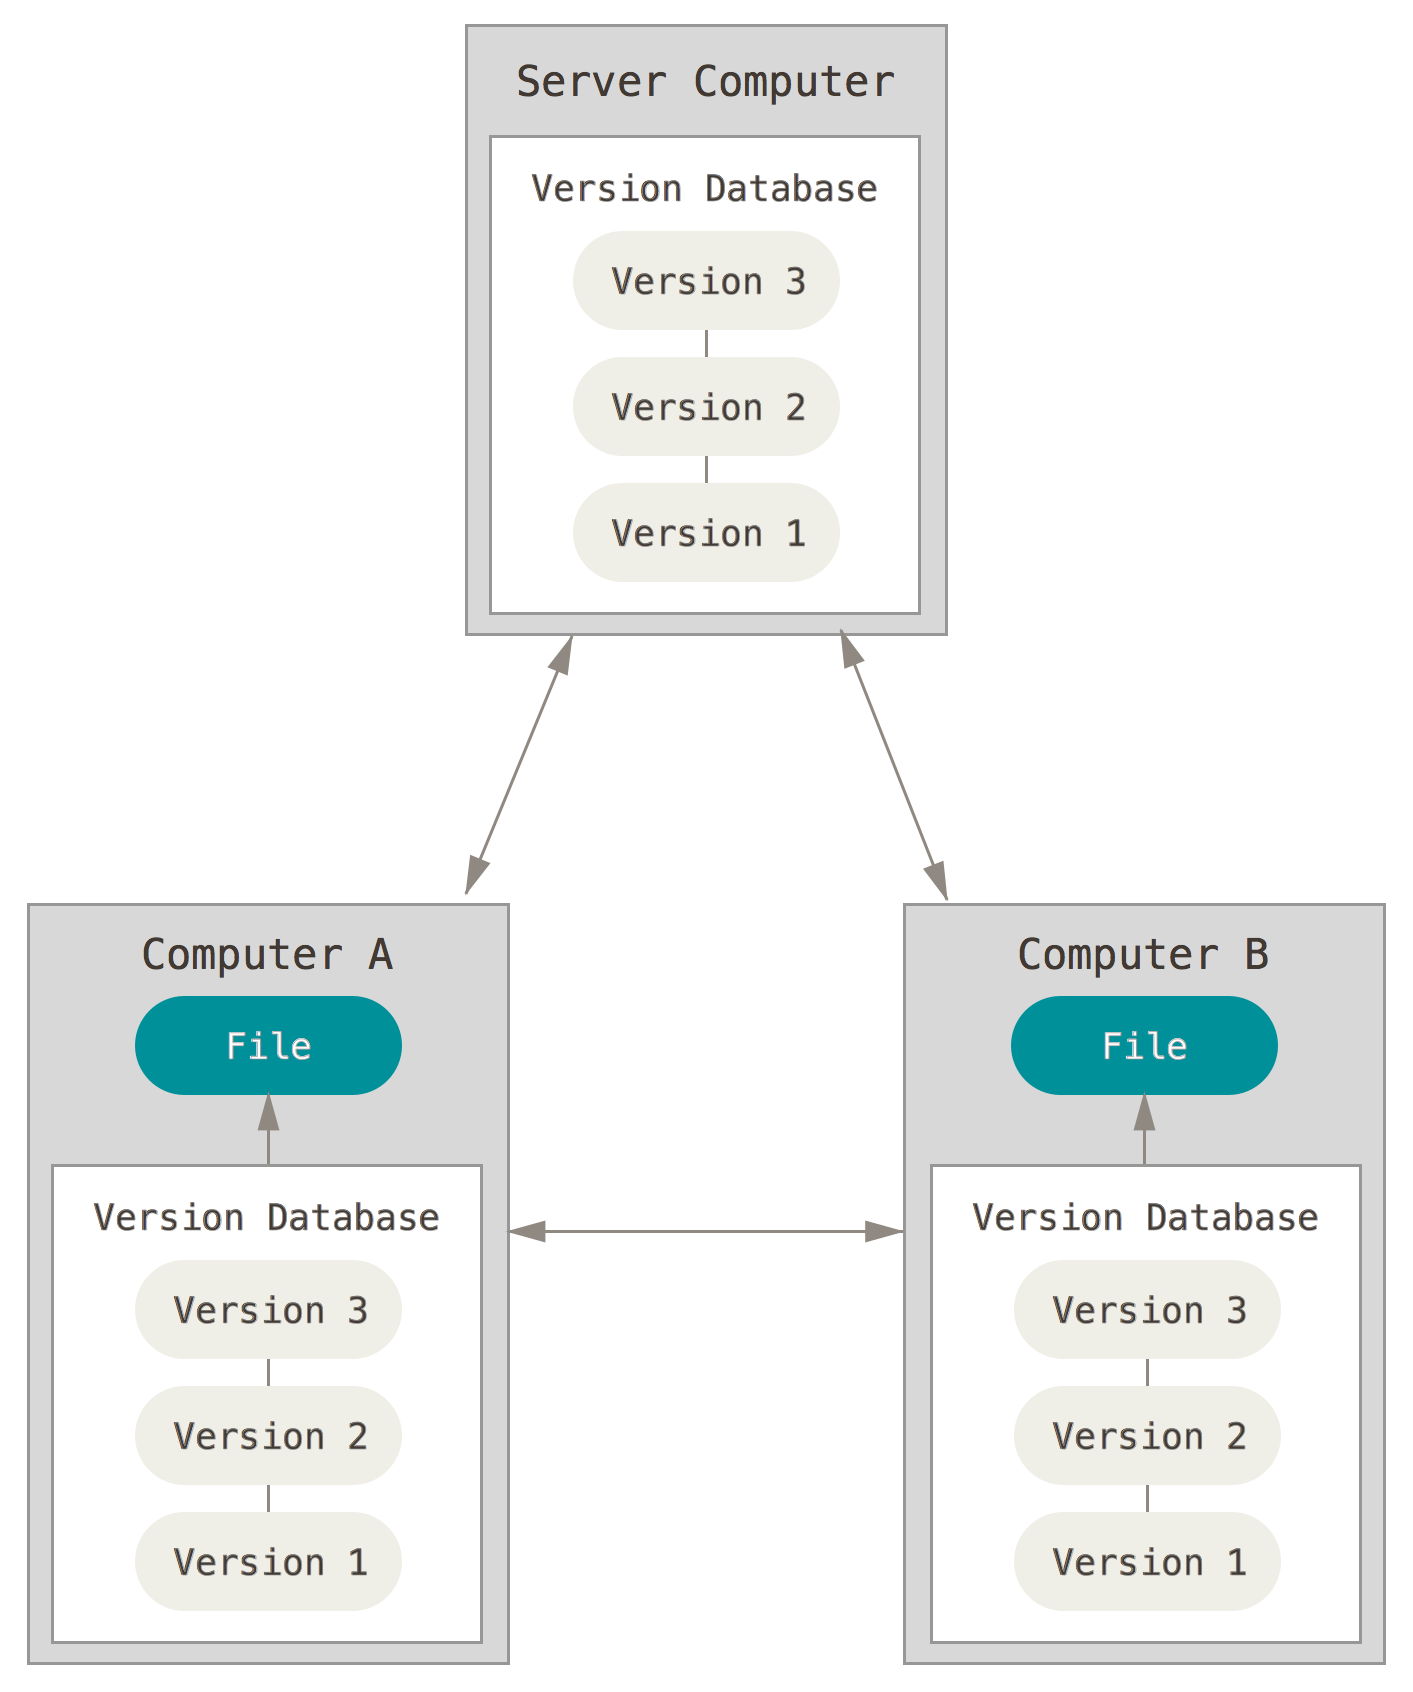
\includegraphics[width=0.5\textwidth]{VersionControlDistributed.png}
	\caption{Dalītas VCS \ref{appfig:VersionControlDistributed}}
	\label{fig:VersionControlDistributed}
\end{figure}
Trešās paudzes VCS piemēri ir \textit{GNU Arch}, \textit{Bazaar}, \textit{Monotone}, \textit{BitKeeper} un \textit{Git}.

\section{Versiju vadības sistēma Git}
% Kas ir repo?
Darbā izmantota Git versiju kontrole. ... % Vēl ko vajag
Git ir DVCS, ko 2005. gadā radīja Linus Torvals kopā ar Linux kodola (angl. \textit{Linux kernel}) izstrādātāju komandu, lai aizvietotu trešās puses DVCS BitKeeper, kuras autori BitMover 2005. gadā izlēma vairs nepiedāvāt bezmaksas versijas Linux kodola izstrādātājiem. Tāpēc Linux kodola izstrādātāji nolēma radīt savu VCS, ko izmantot Linux kodola versiju vadībai. Galvenie mērķi jaunajai sistēmai bija, lai tā būtu ātra, pilnībā dalīta, spētu efektīvi apstrādāt lielus projektus un atbalstītu nelineāru izstrādi.

\subsection{Kā strādā Git}
Git piedāvā līdzīgu lietotāja saskarni kā citas VCS, bet iekšienē Git datus uztver savādāk nekā citas VCS. Lielākā daļa VCS saglabā veikto izmaiņu sarakstu, attiecīgi kā datnes un to izmaiņas, jeb deltas.
% Attēls https://git-scm.com/book/en/v2/Getting-Started-Git-Basics
Toties Git katru versiju uztver gluži kā failu sistēmas momentuzņēmumu. Katra saglabātā versija saglabā esošo projekta stāvokli un, lai sistēma būtu efektīvāka, uz datnēm kuras nav mainītas Git izveido atsauces. Git, uztverot versijas kā failu sistēmas momentuzņēmumus, atļauj ļoti efektīvi veidot nelineāras darbplūsmas (angl. \textit{Workflow}).
% Attēls un arī varētu piemēru no Pluralsight video.
Vēl viens būtisks ieguvums no DVCS ir tas, ka lielākā daļa darbību ir iespējams izdarīt lokāli, bezsaistē. Tas nozīmē, ka Git ir ļoti ātrs, jo nav nekāds tīkla virstēriņš lielākajai daļai darbību, kas ir tipisks CVCS.
% Nearly every operation is local

Integritāte
Pirms Git saglabā datus, tas visam izveido SHA-1 kontrolsummu (angl. \textit{Checksum}) un pēc tam veido atsauces izmantojot izveidotās kontrolsummas. Savā datubāzē Git saglabā visu pēc datņu satura kontrolsummas, nevis pēc to nosaukuma. Tas nozīmē, ka ir neiespējami izdarīt izmaiņas tā, lai Git par tām nezinātu. Tā Git spēj atklāt datu bojājumus, kas radušies tīkla vai cietā diska bojājumu gadījumā. Kā arī, praktiski visas Git darbības tikai pievieno datus datubāzē, tāpēc bieži ir iespējams atgūt datus, kuri šķiet neatgriezeniski pazaudēti.

Trīs stāvokļi
Staging - Ļauj sagatavot savu ``Commit''. Iespējams iekļaut tikai daļu no savām izmaiņām.

\subsection{Zarošanās}
Zarošanās (angl. \textit{Branching})
Git zarošanās ir ļoti spējīgs mehānisms, kas ļauj veikt eksperimentus it nemaz netraucējot jau uzrakstītajam kodam.
\subsubsection{Izvēlētā zarošanās stratēģija}
% http://nvie.com/posts/a-successful-git-branching-model/
% https://www.atlassian.com/git/tutorials/comparing-workflows/gitflow-workflow
Darbā izvēlēts izmantot Gitflow darbplūsmu, kas ir īpaši lietderīga lieliem projektiem, jo Gitflow darbplūsma skaidri nosaka repozitorija zaru funkcijas. Gitflow pamatā galvenie ir divi zari: pamatzars (angl. \textit{master}) un izstrādes zars(angl. \textit{develop}). Pamatzars atspoguļo relīžu vēsturi un koda iesūtījumi ir atzīmēti ar versiju numuriem. Ikreizi, kad pamatzarā tiek veikta kāda izmaiņa, to jāatzīmē ar jaunu versijas numuru. Izstrādes zars kalpo pievienotās funkcionalitātes integrācijai. Tomēr, katrai pievienotajai iespējai vajadzētu atrasties savā funkcionalitātes (angl. \textit{feature}) zarā. Citās darbplūsmās parasti atzarojas no pamatzara, bet Gitflow darbplūsmā atzarošanās tiek veikta no izstrādes zara. Katra jaunā iespēja atzarojas no izstrādes zara un kad tā ir pabeigta, tā tiek sapludināta ar izstrādes zaru.
Kad pienāk laiks jaunai relīzei, no izstrādes zara atzarojas relīzes zars. Relīžu zaros nekad netiek pievienota jauna funkcionalitāte. Relīzes zari tiek tikai izmantoti tālākai koda sagatavošanai nākamajai versijai, tajā veic tikai labojumus. Tajā nepievieno papildus funkcionalitāti. Kad relīze ir gatava, to sapludina ar pamatzaru, atzīmē ar jaunu versijas numuru un sapludina arī ar izstrādes zaru.
Apkopes (angl. \textit{maintenance}) zari tiek izmantoti, lai ātri veiktu labojumus relīzēm. Apkopes zars atzarojas no pamatzara un tiklīdz labojums ir pabeigts, tas tiek sapludināts ar pamatzaru un izstrādes zaru, vai vēl neizlaistu relīzes zaru.
Šāda vairākzaru darbplūsma ļauj izstrādei neapstāties pie viena uzdevuma, piemēram, nespiež strādāt tikai pie relīzes vai papildu funkcionalitātes izstrādes. Tā kā ir vairāki zari gan relīzēm, gan funkctionalitātei, komandas var strādāt paralēli, katra pie sava uzdevuma nebojājot repozitoriju citām komandām.
Gitflow darbplūsma attēlota \ref{fig:WorkflowGitflow}. Šīs un citu darbplūsmu piemēri atrodami \cite{workflow-comparison}.
\begin{figure}[H]%!ht
	\centering
	\captionsetup{justification=centering}
	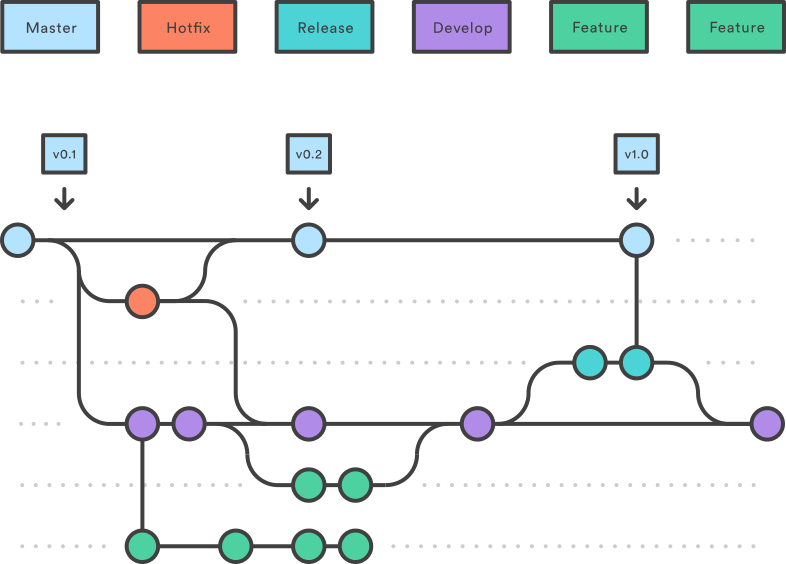
\includegraphics[width=0.5\textwidth]{WorkflowGitflow.png}
	\caption{Gitflow zarošanās stratēģijas attēlojums \ref{appfig:WorkflowGitflow}}
	\label{fig:WorkflowGitflow}
\end{figure}
Master zars atspoguļo to mājaslapas kodu, kas strādās uz RaspberryPi servera. Tiklīdz kā tikt atjaunināts master zars, serveris to lejuplādēs un sāks izmantot jaunāko koda relīzi.
Develop zars izmantots izmaiņu integrēšanai.
Galvenais darbs notiks uz feature zariem, kuros fokusēti tiks nodalīta laika gaitā pievienotā funkcionalitāte.



Darba praktiskā daļa ir sadalīta divos repozitorijos. Viens repozitorijs - piekļuves sistēmas administrēšanas mājaslapai, otrs - infrastruktūras uzstādīšanai izmantojot Chef.

\chapter{Konfigurācijas pārvaldība}
Šajā nodaļā apskatīta konfigurācijas pārvaldības nozīmība un īstenošana izmantojot konfigurācijas pārvaldības rīkju Chef, kas ļauj aprakstīt infrastruktūru kodā.
Konfigurācijas pārvaldība nodrošina vispārēju sistēmas vadību un satur datus no pārvaldāmajiem objektiem. Sākot no 1960' gadiem, konfigurācijas datus saglabāja datu bāzē, ko konfigurācijas pārvaldnieks var izmantot iekārtu - darbstaciju, serveru, maršrutētāju, u.c. - konfigurēšanai.
Konfigurācijas pārvaldība palīdz nodrošināt komponenšu un sistēmas kvalitāti, to atbilstību noteiktajajām tehniskajām prasībām, kā arī palīdz veikt sistēmu auditēšanu.

\section{Infrastruktūra kā kods}
Sistēmas administratori jau izsenis centušies automatizēt sistēmu uzstādīšanu un konfigurēšanu. Ierasts izmantot \textit{bash} skriptus, kuros secīgi sarakstītas izpildāmās komandas, konfigurācijas veikšanai. Laika gaitā tika radīta specializēta programmatūra, kas ļauj infrastruktūru aprakstīt kodā, automatizēt sistēmu uzstādīšanu un konfigurēšanu. Pašlaik populārākie rīki ir 2005. gadā radītais Puppet, 2009. gadā - Chef, 2012. gadā - Ansible. Šie rīki ļauj visu infrasturktūru aprakstīt kodā - sistēmu konfigurāciju, ieskaitot lietotāju pārvaldību. Darbā izmantots konfigurācijas pārvaldības rīks Chef, kas radīts 2009. gadā un ir uzrakstīts izmantojot Ruby un Erlang programmēšanas valodas.
Chef ir spēcīga automatizēšanas platforma, kas apraksta sarežģītu infrastruktūru kodā, neatkarīgi no tā, vai resursi atrodas mākonī\nomenclature{Mākonis}{Mākoņdatošana (angl. \textit{Cloud computing})}, uz lokāliem serveriem vai to kombinācijā. Chef spēj automatizēt kā lietotnes ir konfigurētas, izvietotas, pārvaldītas, neatkarīgi no uzstādītās infrastruktūras izmēra. \cite{chef-docs}
Chef pamatā ir vienkārša koncepcija: vēlamā stāvokļa sasniegšana, centralizētas IT infrastruktūras modelēšana un resursu primitīvi, kas kalpo kā pamatelementi. Šī koncepcija ļauj efektīvi pārvaldīt pat ļoti sarežģītas infrastruktūras.
% Automatizēta, abstahēta, vienkāršota
\subsection{Chef komponentes}
Konfigurācijas orķestrēšanai Chef strādā pēc vedējsekotājsistēmas (angl. \textit{Master-slave system}) principa. Galvenais ir Chef serveris, kurš pārvalda infrastruktūru.
Diagrammā \ref{fig:ChefOverview} redzams Chef komponenšu attiecības starp Chef serveri, mezgliem (angl. \textit{nodes}) un izstrādātāja darbstaciju.
\begin{figure}[H]%!ht
	\centering
	\captionsetup{justification=centering}
	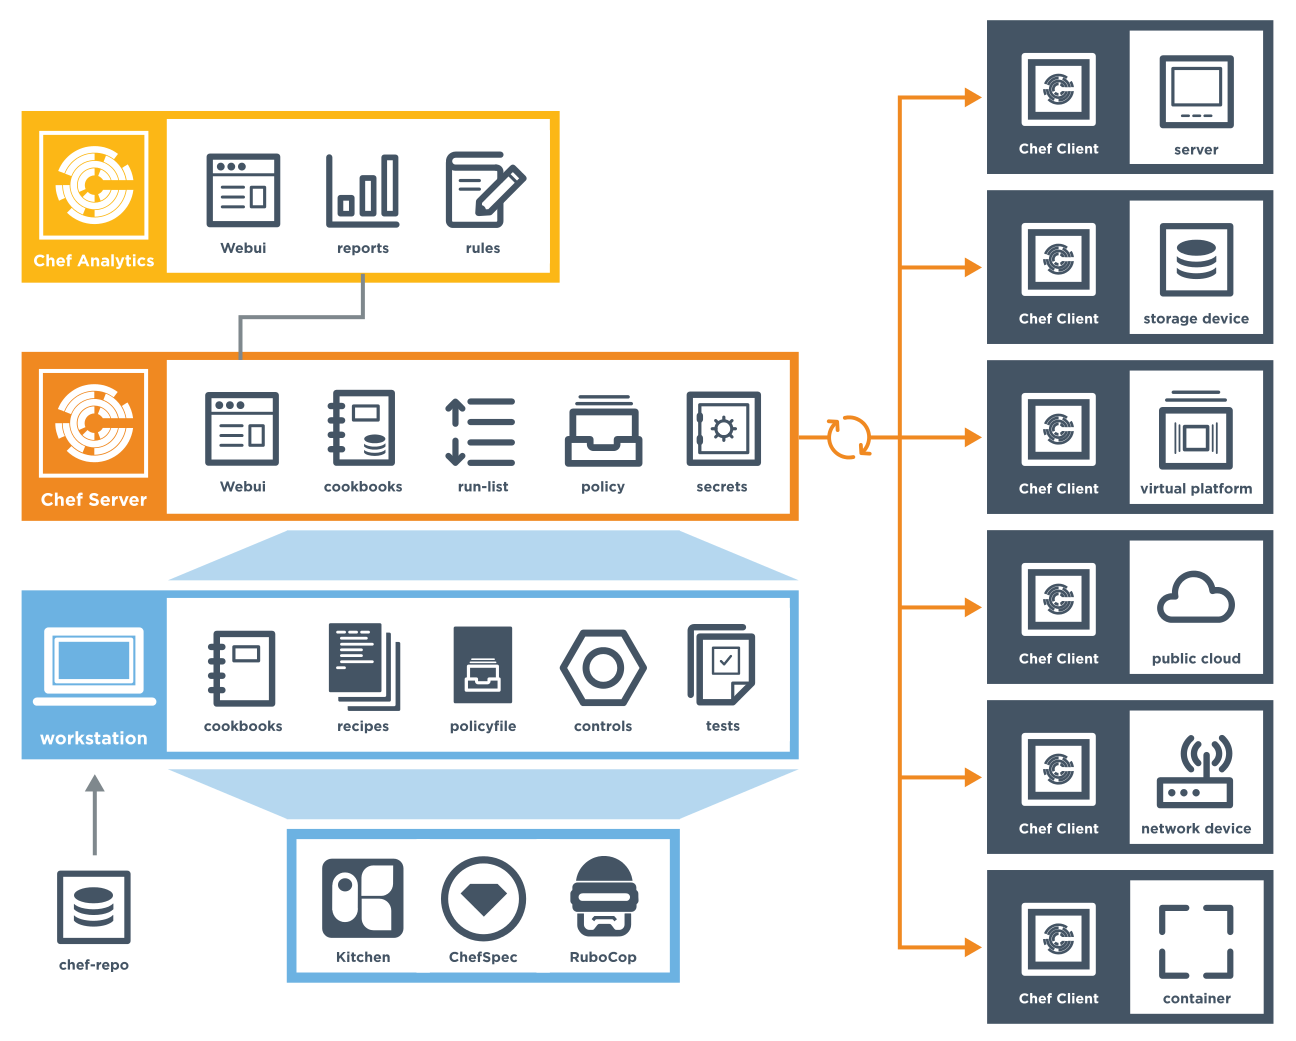
\includegraphics[width=0.5\textwidth]{ChefOverview.png}
	\caption{Chef komponentes \ref{appfig:ChefOverview}}
	\label{fig:ChefOverview}
\end{figure}
Galvenās Chef komponentes:
\begin{itemize}
	\item Izstrādātāja darbstacija, kas ir konfigurēta darbam ar Chef. Minimums, lai sāktu izstrādi ar Chef, ir uzinstalēta Ruby programmēšanas valoda, bet ieteicams izmantot Chef izstrādes rīkkopu (angl. \textit{Chef development kit}), kas satur vēl citas izvēles pakotnes, ieskaitot Chef komandrindas rīku, Kitchen, ChefSpec, Berkshelf, u.c. rīkus.
	\item Chef izmanto domēnam specifisku valodu, lai aprakstītu lielu daļu konfigurācijas, kas balstīta uz Ruby programmēšanas valodu un izmanto tās sintaksi. Chef ir ļoti pielāgojams, jo ļauj pilnībā izmantot Ruby dotās iespējas.
	\item Mezgli - jebkuras sistēmas (fiziskas, virtuālas, mākonis, u.t.t.), ko pārvalda Chef. Chef klients (angl. \textit{chef-client}) ir izpildāma programma, kas uzstādīta uz katra mezgla un tā izpilda visus konfigurācijas uzdevumus.
	\item Chef serveris - kalpo kā centrmezgls. Konfigurācija tiek augšupielādēta uz Chef servera no darbstacijām. Chef klients savienojas ar Chef serveri un saņem tā konfigurācijas datus.
	Chef pārvaldības konsole ir Chef servera lietotāja saskarne, ko lieto, lai pārvaldītu data bags (!!!!!!!!!!!!!!!!!!), rekvizītus, run-lists, lomas, vidi, recepšu grāmatas.
	\item Chef analīze
	\item Chef lielveikals (angl. \textit{Chef Supermarket}) - šeit atrodas brīvi izmantojamas Chef kopienas recepšu grāmatas. Tajā jau ir gandrīz trīs tūkstoši sagatavotu recepšu grāmatu, kuras spēj veikt lielāko daļu konfigurācijas daudziem rīkiem.
\end{itemize}



Chef pamatā galvenais ir Chef repozitorijs, kurā glabājas viss konfigurācijas kods. Izstrādātājs lejuplādē repozitoriju uz lokālās darbstacijas un uz tās veic arī turpmāko izstrādi. Repozitorijā atrodas recepšu grāmatas (angl. \textit{cookbooks}), kurās atrodas receptes (angl. \textit{recipes}).
Izmantojot Chef izstrādes rīkkopu, izstrādātājs uz savas darbstacijas var rakstīt konfigurāciju.
Uzrakstīto kodu ir iespējams arī testēt. Ir iespējams pārbaudīt uzģenerēto datņu, izpildīto komandu atbilstību vēlamajam ar vienību testiem (angl. \textit{unit test}) izmantojot ChefSpec, kā arī testēt ar integrācijas testiem (angl. \textit{integration test}), izmantojot testu virtuvi (angl. \textit{Test Kitchen} \url{http://kitchen.ci/}). Integrācijas testi ļauj pārbaudīt kā viss strādā kopā, jo testu virtuve izveido jaunu sistēmas eksemplāru mākonī vai uz lokālas darbstacijas, izmantojot Vagrant virtuālās mašīnas vai Docker konteinerus. Ir izveidotas arī koda kvalitātes un stila pārbaudes, ko iesaka izmantot vismaz kopienas \textit{cookbooks}, tādejādi cenšoties kopienas \textit{cookbooks} padarīt konsistentākas.
Izmantojot Chef izstrādes rīkkopas rīku \textit{knife}, izstrādātājs lielāko daļu darba var veikt no lokālās darbstacijas. \textit{Knife} ļauj augšuplādēt recepšu grāmatas uz Chef servera, pārvaldīt uzstādītos mezglus, kā arī pievienot jaunus mezglus Chef serverim.

% Ir galvenais Chef serveris uz kura glabājas vairākas komponentes:
% \begin{itemize}
% 	\item recepšu grāmatas (angl. \textit{cookbooks}) - kurās atrodas receptes (angl. \textit{recipes}).
% \end{itemize}
% Chef struktūra
% Chef repozitorijs - nosaka konfigurācijas pārvaldības struktūru. Repozitorijs satur:
% 	Recepšu grāmatas\nomenclature{Cookbooks}{Recepšu grāmatas (angl. \textit{cookbooks}) - satur receptes}
% 		Receptes\nomenclature{Recipes}{Receptes (angl. \textit{recipes}) - tajās konfigurācija tiek aprakstīta kodā.}
% 		Rekvizīti\nomenclature{Attributes}{Rekvizīti (angl. \textit{attributes}) - tie var tikt definēti recepšu grāmatā vai receptē un tos var izmantot, lai pārlabotu noklusējuma iestatījumas uz mezgla.}
% 	Datu somas\nomenclature{Data bags}{Datu somas (angl. \textit{data bags}) - līdzīgi rekvizītiem, tās izmanto noklusēto iestatījumu pārlabošanai. Atšķirībā no rekvizītiem, datu somas ir iespējams šifrēt.}
% 	Vide\nomenclature{Environment}{Vide (angl. \textit{environment}) - katram mezglam ir noteikta vide, ar kuru iespējams noteikt izmantoto recepšu versijas.}
% 	Lomas\nomenclature{Roles}{Lomas (angl. \textit{roles}) }
%
% Chef serveris
% 	Nodes
% 		Chef-client
% 		Run-list
% 			Cookbooks
% 		Attributes
% 		Environment

% Chef struktūra
% \begin{itemize}
% 	\item Chef repozitorijs
% 	\begin{itemize}
% 		\item Cookbooks
% 		\begin{itemize}
% 			\item Recipes
% 			\item Attributes
% 		\end{itemize}
% 		\item Data_bags
% 		\item Environments
% 		\item Roles
% 	\end{itemize}
% 	\item Chef-server
% 	\begin{itemize}
% 		\item Chef repozitorijs
% 		\item Nodes
% 		\begin{itemize}
% 			\item Chef-client
% 			\item Run-list
% 			\item Cookbooks
% 			\item Attributes
% 			\item Environment
% 		\end{itemize}
% 	\end{itemize}
% \end{itemize}

\chapter{Ruby on Rails}
Darbā tika radīta mājaslapa telpas piekļuves administrēšanai izmantojot Ruby on Rails satvaru. Ruby on Rails ir tīmekļa lietojumprogrammu satvars (angl. \textit{web application framework}), kas  sevī ietver visu nepieciešamo, lai radītu ar datubāzi nodrošinātu lietojumprogrammu, kas balstīta uz Modeļa-Skata-Kontroliera \nomenclature{MVC}{Modelis-Skats-Kontrolieris (angl. \textit{Model-View-Controller})} modeļa.

% MVC struktūra ļauj sakārtot kodu un labāk saprast mājaslapas darbību.
MVC sadala lietojumprogrammu trīs slāņos, kur katram slānim ir sava pienākums.
Skata slānis satur šablonus, kurus izmanto, lai sagatavotu mājaslapas izskatu un attēlotu ievadītos datus. Ruby on Rails izmanto HTML šablonus ar integrētu Ruby kodu.
Modelis attēlo domēna modeli (piemēram. Lietotāji, Produkti). Praktiski, lielākā daļā modeļu ir balstīti uz datubāzi un attēlo tās īpašības.
Kontrolieris apstrādā ienākošos HTTP pieprasījumus un dod atbilstošu atbildi. Kontrolieris saņem lietotāja klikšķus, nosūta komandas modelim un galu galā uzģenerē skatus izmantojot iepriekš izveidotos šablonus.
% http://api.rubyonrails.org/

\section{Kāpēc izmantot Ruby on Rails?}
Rails parūpējas par daudz lietām, kas mēdz radīt kļūdas, piemēram Rails veic SQL vaicājumu ģenerēšanu. Izstrādātājam nav jāuztraucas par piekļuvi datubāzei, datu ierakstīšanu un iegūšanu no datubāzes. Rails doktrīnā viens no punktiem ir "Konvencija pāri konfigurācijai" (angl. \textit{Convention over configuration}), tas nozīmē, ka Rails izstrādātājiem ir skaidra ideja, kā pareizi programmēt tīmekļa lietojumprogrammas. Tāpēc daudzas lietas ir abstrahētas, kas būtiski vienkāršo izstrādi, kā arī Rails apgūšanu.

\chapter{Testēšana}
Ir vairāki aplikāciju izsrādes paņēmieni. Viens no paņēmieniem ir testu virzīra izstrāde \nomenclature{TDD}{Testu virzīta izstrāde (angl. \textit{Test driven development})}. TDD sevī ietver testu uzrakstīšanu pirms tiek uzrakstīts aplikācijas kods. Tādejādi TDD pamatprincips ir šāds: Sākumā tiek uzrakstīts tests, kurš neizdodas un pēc tam tiek uzrakstīts tikai tik daudz koda cik nepieciešams, lai tests izpildītos veiksmīgi. Kad tests izpildas

Pēc tam iespējams apskatīt, vai kodu ir iespējams vienkāršot vai uzlabot, nemainot tā funkcionalitāti.
\section{RSpec}
RSpec jeb RubySpec ir populārākā Ruby testēšanas bibliotēka. RSpec tika izdots 2005. gadā.
\cite{shayRspec}

RSpec ir uzvedības virzītas izstrādes (angl. \textit{behavior driven development}) testēšanas satvars. RSpec izmanto savu domēnam specifisku valodu \nomenclature{DSL}{Domēnam specifiska valoda (angl. \textit{Domain specific language})}, kas līdzinās dabiskas valodas specifikācijai. Lasot RSpec testus tiem būtu jāizklausās pēc normāliem teikumiem. Tā RSpec cenšas testus padarīt lasāmus un saprotamus.
\section{Nepārtraukta integrācija}
Nepārtraukta integrācija (angl. \textit{Continuous Integration})
\subsection{TravisCI}


\chapter{Drošība}

\section{Tipiskākie uzbrukumi un to novēršana}
\subsection{SQL injekcija}
\subsection{Cross Site scripting}

\section{RFID sistēmas}
\section{Lietotāja autentiskums}